\section{9758 JC2 Preliminary Examination Paper 1}

\begin{problem}
    It is given that \[2xy \der{y}{x} = x^2 - y^2\] where $x > 0$, $y < 0$. Using the substitution $u = y/x$, show that the differential equation can be transformed to \[\frac{2u}{1 - 3u^2} \der{u}{x} = \frac1x.\] Hence, find the general solution of $y$ in terms of $x$.
\end{problem}
\begin{solution}
    Note that $y = ux$, so \[\der{y}{x} = x \der{u}{x} + u.\] Substituting this into the given differential equation, we get \[2ux^2 \bp{x \der{u}{x} + u} = x^2 - u^2 x^2.\] Since $x \neq 0$, we may divide both sides by $x^2$ to get \[2u\bp{x \der{u}{x} + u} = 1 - u^2,\] which rearranges to \[\frac{2u}{1 - 3u^2} \der{u}{x} = \frac1x.\] Integrating both sides with respect to $x$, we get \[\int \frac{2u}{1 - 3u^2} \d u = \int \frac1x \d x.\] Since $x > 0$, we see that \[-\frac13 \ln \abs{1 - 3u^2} = \ln{x} + C_1.\] Exponentiating both sides, we obtain \[C_2 x = \bp{1 - 3u^2}{-1/3},\] where $C_2 = \pm \e^{C_1}$. Cubing both sides and simplifying, we see that \[C_3 x^3 = \frac1{1-3u^2} = \frac{x^2}{x^2 - 3y^2} \implies y^2 = \frac{C_3 x^3 - 1}{3C_3 x},\] where $C_3 = C_2^3$. Since $y < 0$, we finally have \[y = -\sqrt{\frac{C x^3 - 1}{3C x}},\] where $C \neq 0$ is an arbitrary constant.
\end{solution}

\clearpage
\begin{problem}
    A series is given by \[\sum_{r = 1}^n 2\bp{4-3x}^r\] where $x$ is constant.

    \begin{enumerate}
        \item Explain why this is a geometric series. Determine the range of values of $x$ for the sum to infinity of this series to exist.
        \item Using $x = 1$, and given that \[\sum_{r = 1}^n r^2 = \frac{n(n+1)(2n+1)}{6},\] find \[\sum_{r = 0}^{n-1} \bs{2\bp{4-3x}^r + \bp{r+1}\bp{2r+5}},\] leaving your answer in the form of $n\bp{an^2 + bn + c}$, where $a$, $b$ and $c$ are constants to be determined.
    \end{enumerate}
\end{problem}
\begin{solution}
    \begin{ppart}
        Let $u_r = 2(4-3x)^r$ be the $r$th term in the sequence being summed. Then \[\frac{u_{r+1}}{u_r} = \frac{2(4-3x)^{r+1}}{2(4-3x)^r} = 4-3x,\] which is a constant since $x$ is constant. Thus, $\bc{u_r}$ is in geometric progression and the given series is a geometric series.

        For the sum to infinity to exist, we must have $\abs{4-3x} < 1$, so $1 < x < 5/3$.
    \end{ppart}
    \begin{ppart}
        For $x = 1$, it is clear that \[\sum_{r = 1}^n 2\bp{4-3x}^r = \sum_{r = 1}^n 2 = 2n.\] Next, we have
        \begin{align*}
            \sum_{r = 0}^{n-1} \bp{r+1}\bp{2r+5} &= \sum_{r = 1}^n r(2r+3)\\
            &= \sum_{r = 0}^n \bp{2r^2 + 3r}\\
            &= 2\cdot\frac{n(n+1)(2n+1)}6 + 3\cdot\frac{n(n+1)}{2}.
        \end{align*}
        Hence, the sum in question is
        \begin{align*}
            \sum_{r = 0}^{n-1} \bs{2\bp{4-3x}^r + \bp{r+1}\bp{2r+5}} &= 2n + 2\cdot\frac{n(n+1)(2n+1)}6 + 3\cdot\frac{n(n+1)}{2}\\
            &= n \bp{\frac23 n^2 + \frac52 n + \frac{23}{6}},
        \end{align*}
        so $a = 2/3$, $b = 5/2$ and $c = 23/6$.
    \end{ppart}
\end{solution}

\clearpage
\begin{problem}
    \begin{enumerate}
        \item Find the first three non-zero terms in the Maclaurin series for $\e^x \sin{x + \pi}$.
        \item It is given that the three terms found in part (a) are equal to the first three terms in the series expansion of $ax(1+bx)^c$ for small $x$, where $a$, $b$ and $c$ are constants. Find the exact values of $a$, $b$ and $c$. Use these values to find the coefficient of $x^4$ in the expansion of $ax(1+bx)^c$, giving your answer as a simplified rational number.
    \end{enumerate}
\end{problem}
\begin{solution}
    \begin{ppart}
        We have
        \begin{align*}
            \e^x \sin{x + \pi} &= -\e^x \sin x\\
            &= -\bp{1 + x + \frac{x^2}{2} + \dots}\bp{x - \frac{x^3}{6} + \dots}\\
            &= -x - x^2 - \frac13 x^3 + \dots.
        \end{align*}
    \end{ppart}
    \begin{ppart}
        Note that \[ax(1 + bx)^c = ax\bp{1 + cbx + \frac{c(c-1)}{2} b^2 x^2 + \dots} = ax + abcx^2 + \frac{ab^2c(c-1)}{2} x^3 + \dots.\] Comparing coefficients with (a), we have \[a = -1, \quad abc = -1, \quad ab^2c(c-1)/2 = -1/3.\] Solving, we get $a = -1$, $b = 1/3$ and $c = 3$. Thus, the coefficient of $x^4$ in the expansion of $ax(1 + bx)^c$ is \[\frac{ab^3 c(c-1)(c-2)}{3!} = -\frac1{27}.\]
    \end{ppart}
\end{solution}

\begin{problem}
    A sequence of real numbers $x_1, x_2, x_3, \dots$ satisfies the recurrence relation \[x_{n+1} = \frac{5x_n + 2}{2x_n + 3}\] for all $n \geq 1$.

    \begin{enumerate}
        \item Given that the sequence converges to $l$, find the possible exact values of $l$.
        \item Describe how the sequence behaves when $x_1 = 3$.
        \item Given that $x_5 = 3503/2158$, find the value of $x_1$.
    \end{enumerate}
\end{problem}
\begin{solution}
    \begin{ppart}
        We have \[l = \lim_{n \to \infty} x_{n+1} = \lim_{n \to \infty} \frac{5x_n + 2}{2x_n + 3} = \frac{5l + 2}{2l + 3}.\] Thus, $2l^2 - 2l - 2 = 0$. By the quadratic equation, this gives \[l = \frac{1 \pm \sqrt5}{2}.\]
    \end{ppart}
    \begin{ppart}
        The sequence is decreasing and converges to $(1 + \sqrt5)/2$.
    \end{ppart}
    \begin{ppart}
        Note that \[x_n = \frac{3x_{n+1} - 2}{-2x_{n+1} + 5}.\] Thus, \[x_4 = \frac{563}{344}, \quad x_3 = \frac{91}{54}, \quad x_2 = \frac{15}{8}, \quad x_1 = \frac{29}{10}.\]
    \end{ppart}
\end{solution}

\begin{problem}
    The graphs of $y = f'(x)$ and $y = \abs{f(x)}$ are shown below.

    \begin{center}\tikzsetnextfilename{531}
        \begin{tikzpicture}[trim axis left, trim axis right]
            \begin{axis}[
                domain=-6:6,
                samples = 101,
                axis y line=middle,
                axis x line=middle,
                xtick = {-2, 1.5},
                ytick = \empty,
                xlabel = {$x$},
                ylabel = {$y$},
                ymin=-1,
                ymax=1.5,
                legend cell align={left},
                legend pos=outer north east,
                after end axis/.code={
                    \path (axis cs:0,0) 
                        node [anchor=north east] {$O$};
                    }
                ]
                \addplot[plotRed, domain=1.5:6] {0.75 * (x-1.5) * e^(0.5- 0.5 * (x-1.5)^2)};

                \addplot[plotRed, domain=-6:-0.5] {8/x^3 + 1};

                \addplot[plotRed, domain=0.5:1.5] {-4.8*(1/(x+0.5) - 0.5)};

                \addplot[dotted] {1};

                \addlegendentry{$y = f'(x)$};

                \node[anchor=south east] at (6, 1) {$y=2$};

                \node[anchor=south west] at (0, -1) {$x = 0$};
            \end{axis}
        \end{tikzpicture}
    \end{center}
    \begin{center}\tikzsetnextfilename{532}
        \begin{tikzpicture}[trim axis left, trim axis right]
            \begin{axis}[
                domain=-4:5,
                samples = 101,
                axis y line=middle,
                axis x line=middle,
                xtick = {1, 2.5},
                ytick = \empty,
                xlabel = {$x$},
                ylabel = {$y$},
                ymin=-2,
                ymax=5.5,
                legend cell align={left},
                legend pos=outer north east,
                after end axis/.code={
                    \path (axis cs:0,0) 
                        node [anchor=north east] {$O$};
                    }
                ]
                \addplot[plotRed, domain=2.506:5] {-3.1*e^(-0.5*(x-2.25)^2)+3};

                \addplot[plotRed, domain=1:2.506] {-0.51 * (x-1) * (x-2.506)};

                \addplot[plotRed, domain=-4:-0.8] {-x+4/x^2-1};

                \addplot[plotRed, domain=0.09:1] {x^(-0.8) -1};

                \addplot[dotted] {3};

                \addlegendentry{$y = \abs{f(x)}$};

                \node[anchor=south east] at (4, 3) {$y=3$};
                
                \addplot[dotted] {-1.4*(x+3)};

                \node[anchor=west] at (-3.3, 0.36) {$y = -x-3$};

                \node[anchor=south west] at (0, -2) {$x = 0$};

                \fill (1.753, 0.289) circle[radius=2.5pt];
                \node[anchor=south] at (1.753, 0.289) {$(1.5, -1)$};

                \fill (-2, 2) circle[radius=2.5pt];
                \node[anchor=north] at (-2, 2) {$(-2, 2)$};
            \end{axis}
        \end{tikzpicture}
    \end{center}

    \begin{enumerate}
        \item State the nature of all turning point(s) of the graph of $y = f(x)$.
        \item State the range of values of $x$ where $f$ is decreasing.
        \item Sketch the graph of $y = f(x)$ indicating clearly the equations of the asymptotes, coordinates of the turning point(s) and the intersections with the axes.
        \item On the graph of $y = \abs{f(x)}$, sketch and label a line $y = kx + 3k$, where $k$ is a constant. Hence, state the range of values of $k$ for which there is no real solution to the equation $\abs{f(x)} = kx + 3k$.
    \end{enumerate}
\end{problem}
\begin{solution}
    \begin{ppart}
        There is a maximum point at $(-2, -2)$ and a minimum point at $(1.5, -1)$.
    \end{ppart}
    \begin{ppart}
        $f$ is decreasing for $-2 \leq x \leq 1.5$, $x \neq 0$.
    \end{ppart}
    \clearpage
    \begin{ppart}
        \begin{center}\tikzsetnextfilename{533}
            \begin{tikzpicture}[trim axis left, trim axis right]
                \begin{axis}[
                    domain=-4:5,
                    samples = 101,
                    axis y line=middle,
                    axis x line=middle,
                    xtick = {1, 2.5},
                    ytick = \empty,
                    xlabel = {$x$},
                    ylabel = {$y$},
                    ymin=-4,
                    ymax=3.5,
                    legend cell align={left},
                    legend pos=outer north east,
                    after end axis/.code={
                        \path (axis cs:0,0) 
                            node [anchor=north east] {$O$};
                        }
                    ]
                    \addplot[plotRed, domain=2.506:5] {-3.1*e^(-0.5*(x-2.25)^2)+3};

                    \addplot[plotRed, domain=1:2.506] {0.51 * (x-1) * (x-2.506)};

                    \addplot[plotRed, domain=-4:-1] {x-4/x^2+1};

                    \addplot[plotRed, domain=0.2:1] {x^(-0.8) -1};

                    \addplot[dotted] {3};

                    \addlegendentry{$y = f(x)$};

                    \node[anchor=north east] at (4, 3) {$y=3$};
                    
                    \addplot[dotted] {1.2 * x+3};

                    \node[anchor=south east] at (-1, 1.6) {$y = x+3$};

                    \node[anchor=south west] at (0, -4) {$x = 0$};

                    \fill (1.753, -0.289) circle[radius=2.5pt];
                    \node[anchor=south] at (1.753, 0) {$(1.5, -1)$};

                    \fill (-2, -2) circle[radius=2.5pt];
                    \node[anchor=south] at (-2, -2) {$(-2, -2)$};
                \end{axis}
            \end{tikzpicture}
        \end{center}
    \end{ppart}
    \begin{ppart}
        \begin{center}\tikzsetnextfilename{534}
            \begin{tikzpicture}[trim axis left, trim axis right]
                \begin{axis}[
                    domain=-4:5,
                    samples = 101,
                    axis y line=middle,
                    axis x line=middle,
                    xtick = {1, 2.5, -3},
                    ytick = \empty,
                    xlabel = {$x$},
                    ylabel = {$y$},
                    ymin=-2,
                    ymax=5.5,
                    legend cell align={left},
                    legend pos=outer north east,
                    after end axis/.code={
                        \path (axis cs:0,0) 
                            node [anchor=north east] {$O$};
                        }
                    ]
                    \addplot[plotRed, domain=2.506:5] {-3.1*e^(-0.5*(x-2.25)^2)+3};

                    \addplot[plotBlue] {x + 3};

                    \addplot[plotRed, domain=1:2.506] {-0.51 * (x-1) * (x-2.506)};

                    \addplot[plotRed, domain=-4:-0.8] {-x+4/x^2-1};

                    \addplot[plotRed, domain=0.09:1] {x^(-0.8) -1};

                    \addplot[dotted] {3};

                    \addlegendentry{$y = \abs{f(x)}$};

                    \addlegendentry{$y = kx + 3k$};

                    \node[anchor=south east] at (4, 3) {$y=3$};
                    
                    \addplot[dotted] {-1.4*(x+3)};

                    \node[anchor=west] at (-3.3, 0.36) {$y = -x-3$};

                    \node[anchor=south west] at (0, -2) {$x = 0$};

                    \fill (1.753, 0.289) circle[radius=2.5pt];
                    \node[anchor=south] at (1.753, 0.289) {$(1.5, -1)$};

                    \fill (-2, 2) circle[radius=2.5pt];
                    \node[anchor=north] at (-2, 2) {$(-2, 2)$};
                \end{axis}
            \end{tikzpicture}
        \end{center}

        For there to be no real solution to the equation $\abs{f(x)} = kx + 3k$, the graphs of $y = \abs{f(x)}$ and $y = kx + 3k$ must not intersect. Thus, $-1 \leq k < 0$.
    \end{ppart}
\end{solution}

\begin{problem}
    A curve $C$ is defined parametrically by \[x = a \tan t, \quad y = a \sec^2 t \sin t, \quad -\frac\pi4 < t < \frac\pi4,\] where $a$ is a positive constant.

    \begin{enumerate}
        \item Show that \[\frac{\tan t}{\sqrt{1 + \tan^2 t}} = \sin t.\]
        \item By using part (a) or otherwise, find the Cartesian equation of $C$ in the form $y = f(x)$, simplifying your answer.
        \item Show that $f(-x) = -f(x)$. Hence, sketch $C$.
        \item Find the exact area of the region bounded by $C$, the $x$-axis and the lines $x = -A$ and $x = A$, leaving your answer in terms of $A$ and $a$.
    \end{enumerate}
\end{problem}
\clearpage
\begin{solution}
    \begin{ppart}
        Note that $\sec t > 0$ on the interval $-\pi/4 < t < \pi/4$. Thus, \[\frac{\tan t}{\sqrt{1 + \tan^2 t}} = \frac{\tan t}{\sqrt{\sec^2 t}} = \frac{\tan t}{\sec t} = \frac{\sin t / \cos t}{1/\cos t} = \sin t.\]
    \end{ppart}
    \begin{ppart}
        Note that $\tan t = x/a$. Thus,
        \begin{align*}
            y &= a \sec^2 t \sin t\\
            &= a \bp{1 + \tan^2 t} \bp{\frac{\tan t}{\sqrt{1 + \tan^2 t}}}\\
            &= a \tan t \sqrt{1 + \tan^2 t} \\
            &= x \sqrt{1 + \frac{x^2}{a^2}}\\
            &= \frac{x\sqrt{x^2 + a^2}}{a}.
        \end{align*}
    \end{ppart}
    \begin{ppart}
        Observe that \[f(-x) = \frac{(-x)\sqrt{(-x)^2 + a^2}}{a} = -\frac{x\sqrt{x^2 + a^2}}{a} = -f(x).\]

        \begin{center}\tikzsetnextfilename{535}
            \begin{tikzpicture}[trim axis left, trim axis right]
                \begin{axis}[
                    domain=-1:1,
                    samples = 101,
                    axis y line=middle,
                    axis x line=middle,
                    xtick = \empty,
                    ytick = \empty,
                    xlabel = {$x$},
                    ylabel = {$y$},
                    ymin=-1.8,
                    ymax=1.8,
                    xmin=-1.4,
                    xmax=1.4,
                    legend cell align={left},
                    legend pos=outer north east,
                    after end axis/.code={
                        \path (axis cs:0,0) 
                            node [anchor=north east] {$O$};
                        }
                    ]
                    \addplot[plotRed] {x*sqrt(x^2 + 1)};

                    \addlegendentry{$y = f(x)$};

                    \draw (1, 1.414) circle[radius=2.5pt];
                    \node[anchor=south] at (1, 1.414) {$(a, \sqrt2 a)$};

                    \draw (-1, -1.414) circle[radius=2.5pt];
                    \node[anchor=south] at (-1, -1.414) {$(-a, -\sqrt2 a)$};
                \end{axis}
            \end{tikzpicture}
        \end{center}
    \end{ppart}
    \begin{ppart}
        Since $y = f(x)$ is odd, the required area is
        \begin{align*}
            \area &= 2 \int_0^A f(x) \d x\\
            &= 2\int_0^A \frac{x \sqrt{x^2 + a^2}}{a} \d x\\
            &= \frac1a \evalint{\frac23 \bp{x^2 + a^2}^{3/2}}{0}{A}\\
            &= \frac{2}{3a} \bp{A^2 + a^2}^{3/2} - \frac{2a^2}{3} \units[2].
        \end{align*}
    \end{ppart}
\end{solution}

\begin{problem}
    The function $f$ is defined by \[f : x \mapsto \e^x + \frac1{2x+2}\] for $x \in \RR$, $x \neq -1$.

    A function $g$, defined for $x \in \RR$, $x \geq 1$ is such that its first derivative is always positive, and $g(1) = -0.5$.

    \begin{enumerate}
        \item Explain why the composite function $fg$ exists.
        \item Given that \[fg(x) = \frac{x}{\sqrt{\e}} + \frac1{2 \ln x + 1},\] find an expression for $g(x)$ in terms of $x$.
        \item The domain of $f$ is now further restricted to $x > k$. State the least value of the integer $k$ for which the function $\inv f$ exists.
    \end{enumerate}

    For the rest of the question, use the value of $k$ found in part (c).

    \begin{enumerate}
        \setcounter{enumi}{3}
        \item Without finding $\inv f$,
        \begin{enumerate}
            \item sketch, on the same diagram, the graphs of $f$, $\inv f$ and $f \inv f$, showing clearly the relationships between the graphs, and
            \item find the gradient of the tangent of the graph of $y = \inv f(x)$ at $x = \e + \frac14$.
        \end{enumerate}
    \end{enumerate}
\end{problem}
\begin{solution}
    \begin{ppart}
        Since $g'(x) > 0$, it follows that $g$ is increasing. Thus, for all $x \geq 1$, we have $g(x) \geq g(1) = -1/2$. Thus, the range of $g$ is a subset of $[-1/2, \infty)$. Since the domain of $f$ is $\RR \setminus \bc{-1}$, it is clear that \[\ran g \subseteq \left[-\frac12, \infty\right) \subset \RR \setminus \bc{-1} = \dom f.\] Thus, $fg$ exists.
    \end{ppart}
    \begin{ppart}
        By observation, $g(x) = \ln x - 1/2$. Indeed, \[fg(x) = \e^{\ln x - 1/2} + \frac1{2\bp{\ln x - 1/2} + 2} = \frac{x}{\sqrt{\e}} + \frac1{2 \ln x + 1}.\]
    \end{ppart}
    \begin{ppart}
        $k = 0$.
    \end{ppart}
    \begin{ppart}
        \begin{psubpart}
            \begin{center}\tikzsetnextfilename{536}
                \begin{tikzpicture}[trim axis left, trim axis right]
                    \begin{axis}[
                        domain=0:5,
                        samples = 101,
                        axis y line=middle,
                        axis x line=middle,
                        xtick = {1.5},
                        ytick = {1.5},
                        xticklabels = {$\frac32$},
                        yticklabels = {$\frac32$},
                        xlabel = {$x$},
                        ylabel = {$y$},
                        ymin=-0.5,
                        ymax=5,
                        xmin=-0.5,
                        xmax=5,
                        legend cell align={left},
                        legend pos=outer north east,
                        after end axis/.code={
                            \path (axis cs:0,0) 
                                node [anchor=north east] {$O$};
                            }
                        ]
                        \addplot[plotRed] {e^x + 1/(2*x + 2)};

                        \addlegendentry{$y = f(x)$};

                        \addplot[plotBlue] ({e^x + 1/(2*x + 2)}, {x});

                        \addlegendentry{$y = \inv f(x)$};

                        \addplot[black, domain=1.5:5] {x};

                        \addlegendentry{$y = f \inv f(x)$};

                        \addplot[dashed, domain=0:1.5] {x};

                        \draw (1.5, 0) circle[radius=2.5pt];
                        \draw (1.5, 1.5) circle[radius=2.5pt];
                        \draw (0, 1.5) circle[radius=2.5pt];

                        \node[anchor=north west] at (1.5, 1.5) {$(\frac32, \frac32)$};
                    \end{axis}
                \end{tikzpicture}
            \end{center}
        \end{psubpart}
        \begin{psubpart}
            Observe that $f(1) = \e + 1/4$. Note also that \[f'(1) = \evalder{\e^x - \frac{2}{(2x + 2)^2}}{x = 1} = \e - \frac{1}{8}.\] Since the graph of $y = \inv f$ is the reflection of $y = f(x)$ about the line $y = x$, it follows that the derivative of $\inv f$ at $x = \e + 1/4$ is \[\frac1{f'(1)} = \frac{1}{\e - 1/8} = \frac{8}{8\e - 1}.\]
        \end{psubpart}
    \end{ppart}
\end{solution}

\begin{problem}
    A complex number $z$ varies with $t$ such that \[z = 2\cos t + \i (3 \sin t),\] where $0 \leq t < 2 \pi$.

    \begin{enumerate}
        \item By taking $x = \Re{z}$ and $y = \Im{z}$, sketch on an Argand diagram the curve that shows that positions of the points representing the complex number $z$. Find the Cartesian equation of this curve.
    \end{enumerate}

    Two complex numbers $z_1$ and $z_2$ for two distinct values of $t$ are such that $\abs{z_1} = \abs{z_2}$ and $0 < \arg{z_1} < \pi/2$.

    \begin{enumerate}
        \setcounter{enumi}{1}
        \item By referring to the Argand diagram in part (a), find the possible values of $\arg{z_1 + z_2}$.
    \end{enumerate}

    It is given further that $z_1$ and $z_2$ are roots to the quadratic equation $z^2 + \a z + \b = 0$.

    \begin{enumerate}
        \setcounter{enumi}{2}
        \item Explain whether it is necessary for $\a$ to be real.
        \item Given that $\a$ is not real and $\abs{z_1} = \abs{z_2} = \sqrt{26}/2$, find the values of $\a$ and $\b$.
    \end{enumerate}
\end{problem}
\begin{solution}
    \begin{ppart}
        \begin{center}\tikzsetnextfilename{537}
            \begin{tikzpicture}[trim axis left, trim axis right]
                \begin{axis}[
                    axis y line=middle,
                    axis x line=middle,
                    xtick = {-2, 2},
                    ytick = {3, -3},
                    yticklabels = {$3\i$, $-3\i$},
                    xmin=-4,
                    xmax=4,
                    ymin=-4,
                    ymax=4,
                    axis equal image,
                    axis on top,
                    xlabel = {$\Re$},
                    ylabel = {$\Im$},
                    legend cell align={left},
                    legend pos=outer north east,
                    after end axis/.code={
                        \path (axis cs:0,0) 
                            node [anchor=north east] {$O$};
                        }
                    ]
            
                    \addlegendimage{plotRed};
                    \addlegendentry{locus of $z$};
                    \draw[plotRed] (0, 0) ellipse[x radius = 2, y radius = 3];
                \end{axis}
            \end{tikzpicture}
        \end{center}

        The Cartesian equation of the curve is \[\frac{x^2}{2^2} + \frac{y^2}{3^2} = 1.\]
    \end{ppart}
    \clearpage
    \begin{ppart}
        \begin{center}\tikzsetnextfilename{538}
            \begin{tikzpicture}[trim axis left, trim axis right]
                \begin{axis}[
                    axis y line=middle,
                    axis x line=middle,
                    xtick = {-2, 2},
                    ytick = {3, -3},
                    yticklabels = {$3\i$, $-3\i$},
                    xmin=-4,
                    xmax=4,
                    ymin=-4,
                    ymax=4,
                    axis equal image,
                    axis on top,
                    xlabel = {$\Re$},
                    ylabel = {$\Im$},
                    legend cell align={left},
                    legend pos=outer north east,
                    after end axis/.code={
                        \path (axis cs:0,0) 
                            node [anchor=north east] {$O$};
                        }
                    ]
            
                    \addlegendimage{plotRed};
                    \addlegendentry{locus of $z$};
                    \draw[plotRed] (0, 0) ellipse[x radius = 2, y radius = 3];
                    \draw[plotBlue] (0, 0) circle[radius=2.5];

                    \fill (1.48, 2.01) circle[radius=2.5pt] node[anchor=south west] {$z_1$};
                    \draw (-1.48, 2.01) node {$\times$};
                    \draw (-1.48, -2.01) node {$\times$};
                    \draw (1.48, -2.01) node {$\times$};
                \end{axis}
            \end{tikzpicture}
        \end{center}

        Let $z_1 = a + \i b$. There are three possibilities for $z_2$ as represented by the three crosses in the above figure.

        \case{1}[$z_2 = -a + \i b$] Then $\arg{z_1 + z_2} = \arg{2b\i} = \pi/2$.

        \case{2}[$z_2 = -a - \i b$] Then $\arg{z_1 + z_2} = \arg 0$ is undefined.

        \case{3}[$z_3 = a - \i b$] Then $\arg{z_1 + z_2} = \arg{2a} = 0$.

        Thus, the possible values of $\arg{z_1 + z_2}$ are 0, $\pi/2$ or undefined.
    \end{ppart}
    \begin{ppart}
        No. Observe by Vieta's formula that $\a = -(z_1 + z_2)$. Since $z_1$ and $z_2$ need not be conjugate (see case 1 in (b)), it follows that their sum, and thus $\a$, need not be real.
    \end{ppart}
    \begin{ppart}
        Let $z_1 = a + \i b$. Then \[a^2 + b^2 = \abs{z_1}^2 = \frac{26}{2^2}.\] At the same time, from part (a), we have \[\frac{a^2}{2^2} + \frac{b^2}{3^2} = 1.\] Solving the two equations simultaneously, we see that $a^2 = 2$ and $b^2 = 9/2$. Since $z_1$ is in the first quadrant, we have $z_1 = \sqrt2 + 3\i/\sqrt2$.

        Since $\a$ is not real, it follows that $z_2$ is in the second quadrant (see case 1 in (b)). Thus, $z_2 = -\sqrt2 + 3\i /\sqrt2$. Thus, by Vieta's formula, we have \[\a = -\bp{z_1 + z_2} = -3\sqrt{2} \i \quad \tand \quad \b = z_1 z_2 = -\frac{13}{2}.\]
    \end{ppart}
\end{solution}

\begin{problem}
    The point $A$ has coordinates $(1, -2, 4)$ and the plane $\pi_1$ has equation $2x - y + 2z = 5$.

    \begin{enumerate}
        \item Find the exact shortest distance between $A$ and $\pi_1$.
    \end{enumerate}

    The plane $\pi_2$ has equation $x + 3y - az = 3$, where $a$ is a constant.

    \begin{enumerate}
        \setcounter{enumi}{1}
        \item Find the vector equation of the line $l$, which is the line of intersection of $\pi_1$ and $\pi_2$, in terms of $a$.
    \end{enumerate}

    The plane $\pi_3$ has equation $bx - 2y + 4z = 3$, where $b$ is a constant.

    \begin{enumerate}
        \setcounter{enumi}{2}
        \item Show that $(a-6)(b-4) = 0$ if $l$ is parallel to $\pi_3$.
        \item State the conditions that $a$ and $b$ must follows for the three planes to form a triangular prism, where all the planes are non-parallel, and they do not have any point in common. Justify your answer.
    \end{enumerate}
\end{problem}
\begin{solution}
    \begin{ppart}
        Observe that $\pi_1$ is normal to $\cveciiix2{-1}{2}$. Additionally, the point $(1, -1, 1)$ lies on $\pi_1$. Thus, the shortest distance between $A$ and $\pi_1$ is
        \[\text{Shortest distance} = \frac{\abs{\bs{\cveciiix1{-2}{4} - \cveciiix1{-1}{1}} \dotp \cveciiix{2}{-1}{2}}}{\abs{\cveciiix2{-1}{2}}} = \frac73 \units.\]
    \end{ppart}
    \begin{ppart}
        Note that $l$ is normal to both $\cveciiix2{-1}{2}$ and $\cveciix13{-a}$. Thus, the direction vector of $l$ is parallel to \[\cveciii2{-1}{2} \crossp \cveciii13{-a} = \cveciii{a-6}{2a+2}{7}.\] Observe also that $(18/7, 1/7, 0)$ lies on both $\pi_1$ and $\pi_2$, and thus lies on $l$. Hence, $l$ has vector equation \[\vec r = \cveciii{18/7}{1/7}{0} + \l \cveciii{a-6}{2a+2}{7},\] where $\l \in \RR$.
    \end{ppart}
    \begin{ppart}
        If $l$ is parallel to $\pi_3$, then $\cveciiix{a-6}{2a+2}{7}$ must be normal to $\cveciiix{b}{-2}{4}$. Thus, \[0 = \cveciii{a-6}{2a+2}{7} \dotp \cveciii{b}{-2}{4} = (a-6)b - 2(2a+2) + 28 = (a-6)(b-4).\]
    \end{ppart}
    \begin{ppart}
        $\pi_1$ and $\pi_2$ already intersect at $l$. Thus, the three planes have no point in common if $l$ does not intersect $\pi_3$. Thus, for the three planes to form a triangular prism, we must satisfy the following four conditions:
        \begin{enumerate}
            \item $l$ is parallel to $\pi_3$;
            \item $l$ is not on $\pi_3$;
            \item $\pi_1$ is not parallel to $\pi_3$; and
            \item $\pi_2$ is not parallel to $\pi_3$.
        \end{enumerate}

        From (c), the first condition forces $(a-6)(b-4) = 0$, so $a = 6$ or $b = 4$.
        
        The second condition gives \[\cveciii{18/7}{1/7}{0} \dotp \cveciii{b}{-2}{4} \neq 3,\] so $b \neq 23/18$.
        
        The third condition gives \[\cveciii{b}{-2}{4} \neq k\cveciii{2}{-1}{2}\] for all $k \in \RR$. Hence, $k \neq 2$ so $b \neq 4$.

        The fourth condition gives \[\cveciii{b}{-2}{4} \neq k\cveciii{1}{3}{a}\] for all $k \in \RR$. Hence, $k \neq -3/2$, so $b \neq -2/3$ or $a \neq 6$. Note however that $a \neq 6$ cannot hold, else $b = 4$ by the first condition, contradicting the third condition.

        Thus, for all four conditions to be true, we must have $a = 6$ and $b \in \RR \setminus \bc{23/18, 4, -2/3}$.
    \end{ppart}
\end{solution}

\begin{problem}
    \begin{figure}[H]\tikzsetnextfilename{539}
        \centering
        \begin{tikzpicture}[trim axis left, trim axis right]
            \begin{axis}[
                domain = 0:4,
                xmin = 0,
                xmax = 4,
                ymin = 0,
                ymax = 4,
                samples = 101,
                axis y line=middle,
                axis x line=middle,
                xtick = {1, 3},
                ytick = \empty,
                xlabel = {$x$},
                ylabel = {$y$},
                legend cell align={left},
                legend pos=outer north east,
                after end axis/.code={
                    \path (axis cs:0,0) 
                        node [anchor=north east] {$O$};
                    }
                ]
                \addplot[plotRed] {x^2/sqrt(1 + e^x)};
                \addlegendentry{$y = f(x)$};

                \draw (1, 0) -- (1, 0.519) -- (1.25, 0.519);
                \draw (1.25, 0) -- (1.25, 0.737) -- (1.5, 0.737) -- (1.5, 0);
                \draw (2.5, 0) -- (2.5, 1.72) -- (2.75, 1.72);
                \draw (2.75, 0) -- (2.75, 1.85) --  (3, 1.85) -- (3, 0);
                \node at (2, 0.69) {$\dots$};
                \draw[<->] (1, 0.2) -- (1.25, 0.2);
                \node[anchor=south] at (1.125, 0.2) {$h$};
            \end{axis}
        \end{tikzpicture}
    \end{figure}

    The diagram above shows a sketch of the graph of $y = f(x)$ for $x \geq 0$. There are $n$ rectangles each of width $h$ drawn under the curve for $1 \leq x \leq 3$. Each rectangle when rotated through $2\pi$ radians about the $x$-axis, will result in a cylindrical disc. The total volume of the $n$ cylindrical discs $V_1$, can be used to estimate the volume $V$, which is the actual volume generated when the region bounded by the curve, the lines $x = 1$ and $x = 3$, and the $x$-axis is rotated through $2\pi$ radians about the $x$-axis.

    \begin{enumerate}
        \item Show that $V_1$, the total volume of the $n$ cylindrical discs, is given by \[V_1 = \pi h \sum_{r = 0}^{n-1} \bs{f(1+rh)}^2.\] State the value of $h$ in terms of $n$.
        \item From the above diagram, it can be observed that $V_1 < V$. Write down $V_2$, a similar expression as $V_1$, where $V_2 > V$.
    \end{enumerate}

    It is now given that $f(x) = x^2/\sqrt{1 + \e^x}$ for $x \geq 0$.

    \begin{enumerate}
        \setcounter{enumi}{2}
        \item Find the value of $\lim_{n \to \infty} V_1$.
        \item Find the area of the region bounded by $y = f(x)$ and another curve with equation $(x-1)^2 + (y-3)^2 = 9$, for $y \leq 3$.
    \end{enumerate}
\end{problem}
\clearpage
\begin{solution}
    \begin{ppart}
        Observe that the radius of the $r$th disc if $f(1 + rh)$, where $r = 0, 1, \dots, n-1$. Thus, the volume of the $r$th disc is $\pi h \bs{f(1+rh)}^2$. Summing over $r = 0$ to $r = n-1$, we see that \[V_1 = \pi h \sum_{r = 0}^{n-1} \bs{f(1+rh)}^2\] as desired.
    \end{ppart}
    \begin{ppart}
        Taking the right-hand Riemann sum, we have \[V_2 = \pi h \sum_{r = 1}^n \bs{f(1 + rh)}^2.\]
    \end{ppart}
    \begin{ppart}
        As $n \to \infty$, the Riemann sum converges to an integral. Thus, \[\lim_{n \to \infty} V_1 = \pi \int_1^3 \bs{f(x)}^2 \d x = 12.3 \tosf{3}.\]
    \end{ppart}
    \begin{ppart}
        \begin{figure}[H]\tikzsetnextfilename{540}
            \centering
            \begin{tikzpicture}[trim axis left, trim axis right]
                \begin{axis}[
                    domain = 0:4,
                    xmin = 0,
                    xmax = 4,
                    ymin = 0,
                    ymax = 4,
                    samples = 101,
                    axis y line=middle,
                    axis x line=middle,
                    xtick = {0.338, 3.87},
                    ytick = \empty,
                    xlabel = {$x$},
                    ylabel = {$y$},
                    legend cell align={left},
                    legend pos=outer north east,
                    after end axis/.code={
                        \path (axis cs:0,0) 
                            node [anchor=north east] {$O$};
                        }
                    ]
                    \addplot[plotRed] {x^2/sqrt(1 + e^x)};
                    \addlegendentry{$y = f(x)$};

                    \addplot[plotBlue] {3 - sqrt(9 - (x-1)^2)};
                    \addlegendentry{$y = 3 - \sqrt{9 - (x-1)^2}$};

                    \fill (0.338, 0.0739) circle[radius=2.5pt];
                    \fill (3.87, 2.14) circle[radius=2.5pt];

                    \draw[dashed] (0.338, 0.0739) -- (0.338, 0);
                    \draw[dashed] (3.87, 2.14) -- (3.87, 0);
                \end{axis}
            \end{tikzpicture}
        \end{figure}
        Since $y \leq 3$, the second curve has equation $y = 3 - \sqrt{9 - (x-1)^2}$. Using G.C., the two curves intersect at $(0.338, 0.0739)$ and $(3.87, 2.14)$. Thus, the area enclosed by the two curves is \[\area = \int_{0.338}^{3.87} \bp{\frac{x^2}{\sqrt{1 + \e^x}} - \bp{3 - \sqrt{9 - (x-1)^2}}} \d x = 3.01 \units[3] \tosf{3}.\]
    \end{ppart}
\end{solution}

\begin{problem}
    An aquarist who has a fixed budget of \$$k$ wants to make a goldfish sanctuary. His design of the tank consists of a circular cover, a cylinder of length $L$ cm and a hemispherical base of radius $r$ cm neatly fitted together. The costs of the material per cm$^2$ used for the cover, the cylindrical surface and hemispherical base are \$20, \$10 and \$30 respectively. Assume that the tank is made of material with negligible thickness.

    \begin{center}\tikzsetnextfilename{541}
        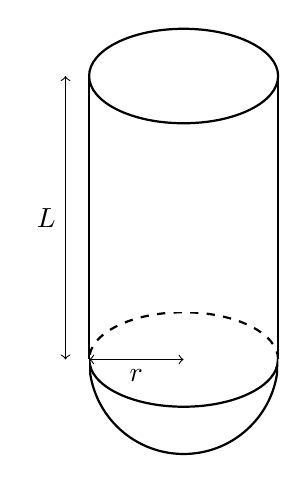
\begin{tikzpicture}[scale=0.6]
            \draw[thick] (0, 0) ellipse[x radius = 2, y radius = 1];
            \draw[thick] (-2, 0) -- (-2, -6);
            \draw[thick] (2, 0) -- (2, -6);
            
            \begin{scope}
                \clip(-2,-7.2)rectangle(2,-6);
                \draw[thick] (0,-6) ellipse[x radius = 2, y radius = 1];
            \end{scope}

            \begin{scope}
                \clip(-2,-6.2)rectangle(2,-5);
                \draw[thick, dashed] (0,-6) ellipse[x radius = 2, y radius = 1];
            \end{scope}

            \begin{scope}
                \clip(-2,-8.2)rectangle(2,-6);
                \draw[thick] (0,-6) circle[radius = 2];
            \end{scope}

            \draw[<->] (-2.5, 0) -- (-2.5, -6);
            \node[anchor=east] at (-2.5, -3) {$L$};

            \draw[<->] (-2,-6) -- (0, -6);
            \node[anchor=north] at (-1,-6) {$r$};
        \end{tikzpicture}
    \end{center}

    \begin{enumerate}
        \item Show that the volume of the tank is $V$ cm$^3$, where \[V = \frac{k}{20} r - \frac{10}{3} \pi r^3.\]
        \item As $r$ varies, find the cost of the material used to make the hemispherical base in terms of $k$ when $V$ is at its maximum value. You need to show that $V$ is a maximum.
    \end{enumerate}

    The aquarist has fixed the radius of the cylinder to be 15 cm. Initially, there is some water in the hemispherical part of the tank. However, due to a defect in the tank, water is leaking at a constant rate of 20 cm$^3$ per minute.
    
    The depth of the water at the hemispherical bottom is denoted by $h$ cm, and the radius of the water surface is $x$ cm. The volume of water in the hemispherical bottom is given by $W$ cm$^3$, where \[W = \frac{\pi h \bp{3x^2 + h^2}}{6}.\]

    \begin{center}\tikzsetnextfilename{542}
        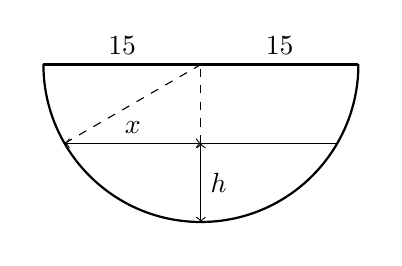
\begin{tikzpicture}
            \begin{scope}
                \clip(-2.2,-2.2)rectangle(2.2,0);
                \draw[thick] (0,0) circle[radius = 2];
            \end{scope}
            \draw[thick] (-2, 0) -- (2, 0);
            \draw[dashed] (-1.73,-1) -- (0, 0);
            \draw[<->] (-1.73, -1) -- (0, -1);
            \draw (0, -1) -- (1.73, -1);
            \draw[<->] (0, -1) -- (0, -2);
            \draw[dashed] (0, -1) -- (0, 0);

            \node[anchor=west] at (0,-1.5) {$h$};
            \node[anchor=south] at (-0.866, -1) {$x$};
            \node[anchor=south] at (-1, 0) {15};
            \node[anchor=south] at (1, 0) {15};
        \end{tikzpicture}
    \end{center}

    \begin{enumerate}
        \setcounter{enumi}{2}
        \item By formulating a relationship between $x$ and $h$, find, when $h = 3$, the rate of change of
        \begin{enumerate}
            \item the depth of water,
            \item the radius of the water surface.
        \end{enumerate}
    \end{enumerate}
\end{problem}
\begin{solution}
    \begin{ppart}
        The total cost is given by \[\bp{20} \bp{\pi r^2} + \bp{10} \bp{2\pi r L} + \bp{30}\bp{2\pi r^2} = k.\] Solving for $L$, we see that \[L = \frac{k}{20 \pi r} - 4r.\] Thus, 
        \begin{align*}
            V &= \pi r^2 L + \frac23 \pi r^3\\
            &= \pi r^2 \bp{\frac{k}{20 \pi r} - 4r} + \frac23 \pi r^3\\
            &= \frac{k}{20} r - \frac{10}{3} \pi r^3.
        \end{align*}
    \end{ppart}
    \begin{ppart}
        For stationary points, $\derx{V}{r} = 0$. Thus, \[\der{V}{r} = \frac{k}{20} - 10 \pi r^2 = 0.\] Solving, we get $r^2 = k/200\pi$. Additionally, \[\der[2]{V}{r} = -20 \pi r < 0\] for all $r > 0$, hence $V$ attains a maximum when $r^2 = k/200\pi$. The desired cost is hence \[30\bp{2\pi r^2} = 30 \bs{2\pi \bp{\frac{k}{200\pi}}} = \$\frac{3}{10} k.\]
    \end{ppart}
    \begin{ppart}
        By Pythagoras' Theorem, $x^2 + (15-h)^2 = 15^2$. Expanding and rearranging, we get $x^2 = 30 h - h^2$. Substituting this into the given formula for $W$, we have \[W = \frac{\pi h \bp{3x^2 + h^2}}{6} = \frac{\pi \bp{45h^2 - h^3}}{3}.\] At $h = 3$, we are given that $\derx{W}{t} = -20$, where $t$ is the time elapsed (in minutes). By the chain rule, we thus have \[\der{h}{t} = \der{h}{W} \der{W}{t} = \frac{-20}{\evalder{\frac\pi{3} \bp{90 h - 3h^2}}{h = 3}} = -\frac{20}{81 \pi}.\] Thus, the depth of the water is decreasing at a rate of $20/81\pi$ cm per minute at $h = 3$.
    \end{ppart}
    \begin{ppart}
        Note that $x = \sqrt{30h - h^2}$ since $x > 0$. By the chain rule, we hence have \[\der{x}{t} = \der{x}{h} \der{h}{t} = \evalder{\frac{15 - h}{\sqrt{30h-h^2}}}{h=3} \bp{-\frac{20}{81\pi}} = -\frac{80}{243\pi}.\] Thus, the radius of the water surface is decreasing at a rate of $80/243\pi$ cm per minute at $h = 3$.
    \end{ppart}
\end{solution}